\documentclass{beamer}
\usepackage{graphicx}
\usepackage{tikz}
\usetikzlibrary{shapes,arrows}
\usepackage{tikz}
%\usecolortheme{seahorse}
\usepackage[makeroom]{cancel}

  \setbeamertemplate{footline}[page number]
\setbeamertemplate{navigation symbols}{}
\setbeamertemplate{frametitle}[default][center]
\setbeamerfont{frametitle}{shape=\scshape}

\usepackage{color}

\usepackage{media9}%
\newcommand{\includemovie}[3]{%
\includemedia[%
width=#1,height=#2,%
activate=pagevisible,%
deactivate=pageclose,%
addresource=#3,%
flashvars={%
src=#3 % same path as in addresource!
&autoPlay=true % default: false; if =true, automatically starts playback after activation (see option ?activation)?
&loop=true % if loop=true, media is played in a loop
&controlBarAutoHideTimeout=0 %  time span before auto-hide
}%
]{}{StrobeMediaPlayback.swf}}%


{\title{\textsc{Numerical Methods-Lecture 11:\\ Neoclassical Growth Model} \\ \ \\ \tiny (See Conesa, Kehoe, Ruhl 2007)}
\author{Trevor Gallen}
\date{}

\begin{document}

\begin{frame}
\titlepage
\end{frame}


%\begin{frame}
%\frametitle[alignment=center]{Agenda}
%\begin{itemize}
%\item Prowse
%\item Idea generation
%\item Presentations \& Guidelines
%\item Roy models \& inefficiency
%\item Code from Sargent \& Ljungqvist
%\item NCG
%\begin{itemize}
%\item Functional forms
%\item Calibration
%\end{itemize}
%\item Solution method
%\item Model meets data
%\end{itemize}
%\end{frame}

%\begin{frame}
%\frametitle[alignment=center]{Idea Generation}
%\begin{itemize}
%\item<1-> Read newspapers, be judgy.
%\item<2-> Read sociology journals, fix them
%\item<3-> Read political science journals
%\item<4-> Read the Statistical Abstract of the U.S.
%\item<5-> Read lists and summaries of laws
%\item<6-> Take advantage of friends \& family members
%\item<7-> Take an hour each day to try to think of new ideas
%\item<8-> Idea journal
%\item<9-> Talk to your friends in the program, pitch ideas
%\item<10-> Put everything into an economics context
%\item<11-> Not to do: read a lot of literature very densely
%\item<12-> Not to do: read a lot of literature on your topic before you do your model
%\item<13-> Not to do: make your paper a slight modification of everyone else's paper
%\item<14-> Choose your question carefully: if time is short, the answer must be interesting no matter what
%\end{itemize}
%\end{frame}

\begin{frame}
\frametitle[alignment=center]{Guidelines on Presentation \& Paper}
\begin{itemize}
\item Pick a topic
\bigskip
\item Pick/write down a model that encompasses what you're talking about
\bigskip
\begin{itemize}
\item Things in your model should be in there for a reason
\bigskip
\item Things not in your model should be excluded for a reason
\bigskip
\end{itemize}
\item Solve your model
\bigskip
\item \emph{Answer a question}.  
\bigskip
\item The presentation \& paper  
\begin{itemize}
\item Motivation (\color<2->{red}{why important})
\item \color<2->{black}{Brief lit review/alternative models}
\item \color<2->{red}{Model}
\item \color<2->{black}{Solution method}
\item Solutions/\color<2->{red}{interesting results}
\item \color<2->{black}{Conclusion}
\end{itemize}
\end{itemize}
\end{frame}


\begin{frame}
\frametitle[alignment=center]{Blanchard's Triangle}
\begin{figure}
\centering
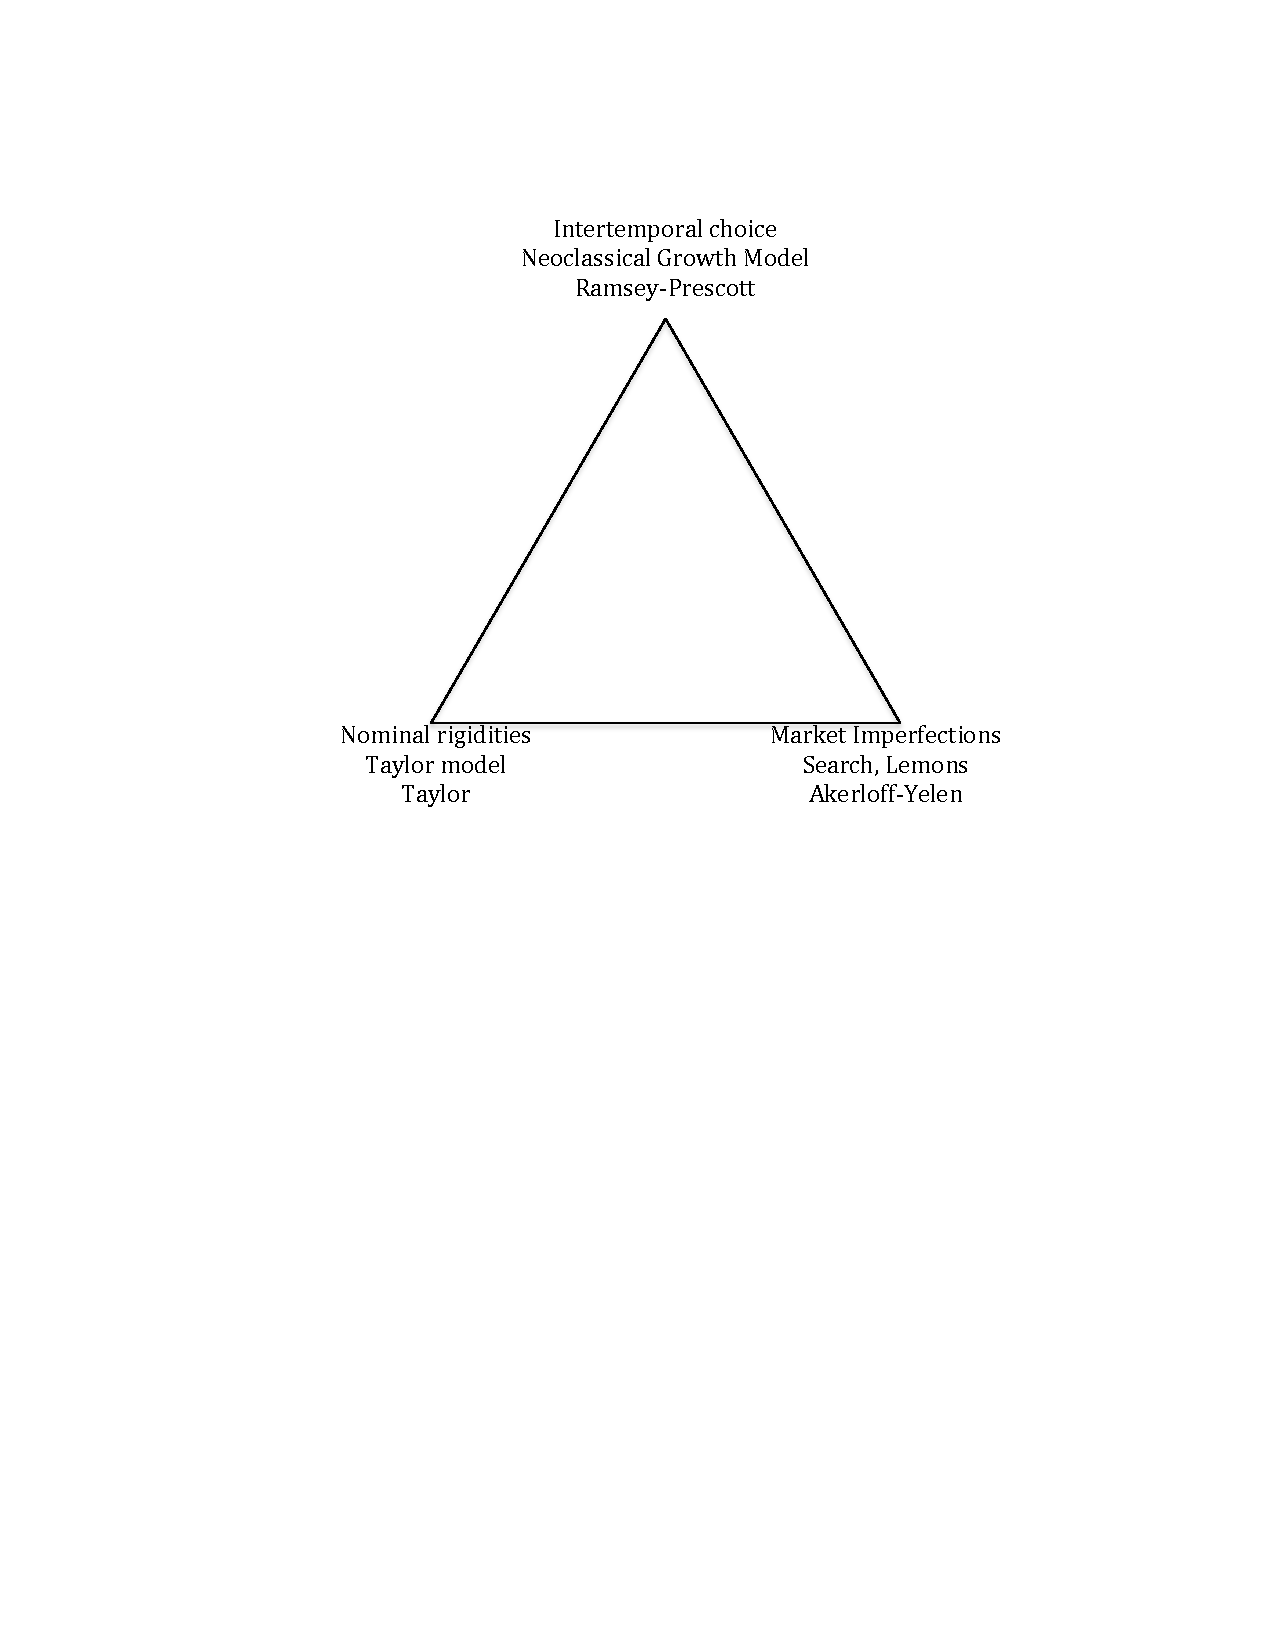
\includegraphics[scale=0.80]{Figures/BlanchardsTriangle-1.pdf}
\end{figure}
\end{frame}

\begin{frame}
\frametitle[alignment=center]{Blanchard's Triangle}
\begin{figure}
\centering
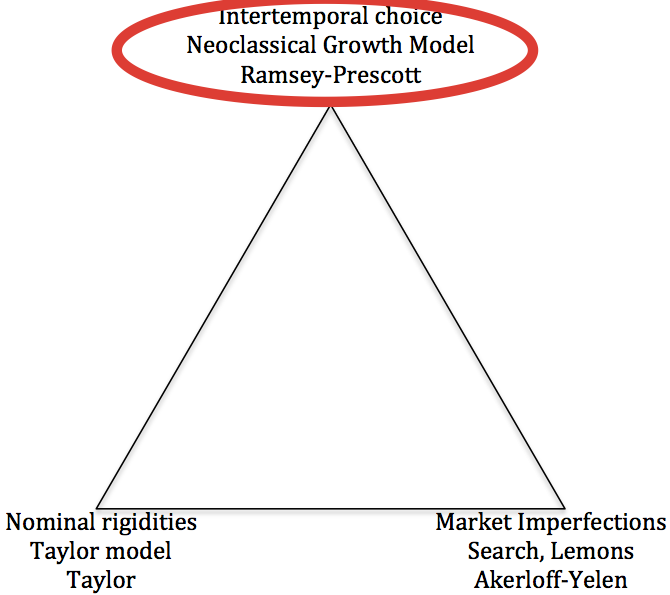
\includegraphics[scale=0.80]{Figures/BlanchardsTriangle-2.png}
\end{figure}
\end{frame}

\begin{frame}
\frametitle[alignment=center]{Neoclassical Growth Model}
\begin{itemize}
\item This is a computational economics course
\bigskip
\item It's worth understanding the NCG
\bigskip
\item Focus on intertemporal choice and consequent dynamics mean an enormous amount of computational models center on it
\end{itemize}
\end{frame}

\begin{frame}
\frametitle[alignment=center]{Neoclassical Growth Model}
\begin{itemize}
\item Utility over consumption and leisure:
$$\sum_{t=0}^\infty \beta^tu(C_t,1-L_t)$$
\item Law of motion
$$C_t+I_t=Y_t=F(K_t,L_t)$$
\item Law of motion of capital
$$K_{t+1}=(1-\delta)K_t+I_t$$
\end{itemize}
\end{frame}

\begin{frame}
\frametitle[alignment=center]{Motivating functional form-I}
\begin{figure}
\centering
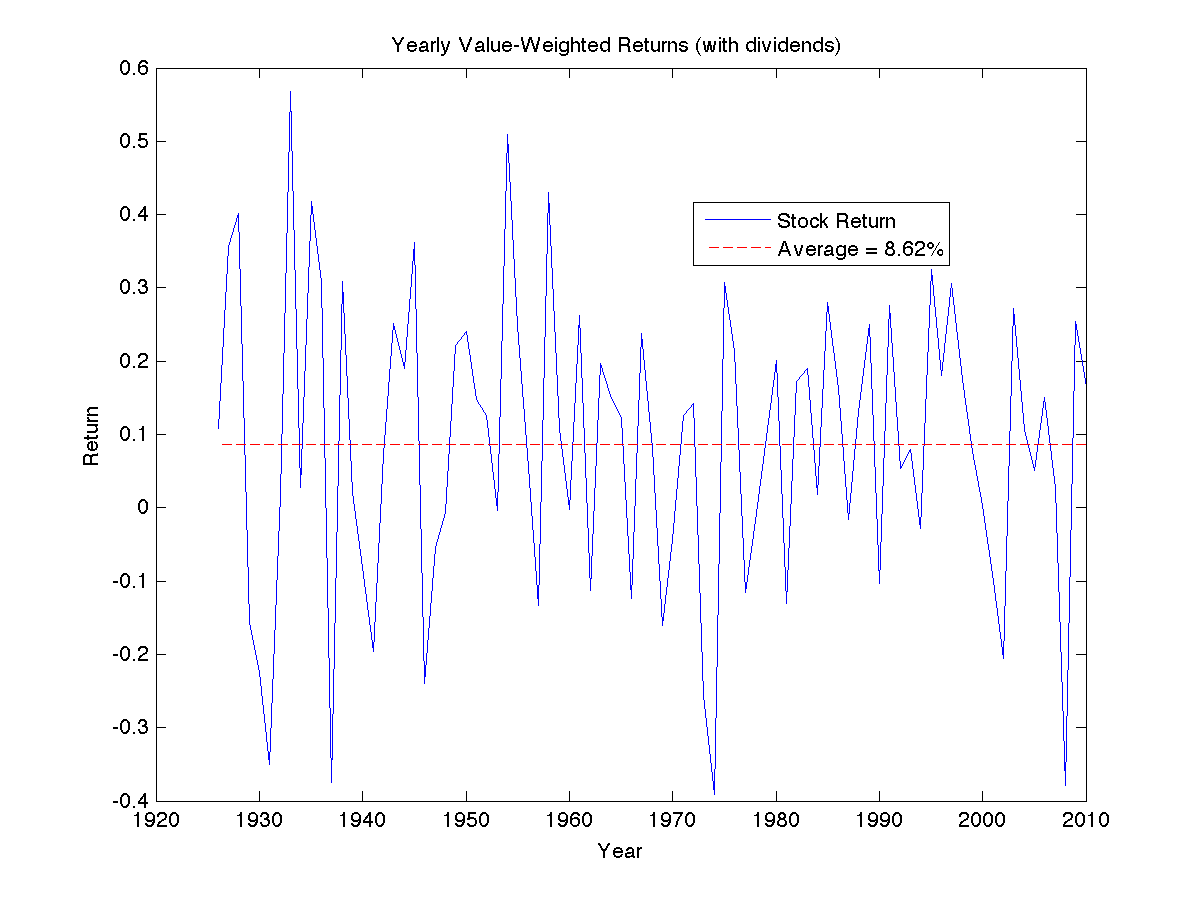
\includegraphics[scale=0.2]{Figures/AnnualReturns}
\end{figure}
\end{frame}

\begin{frame}
\frametitle[alignment=center]{Motivating functional form-II}
\begin{figure}
\centering
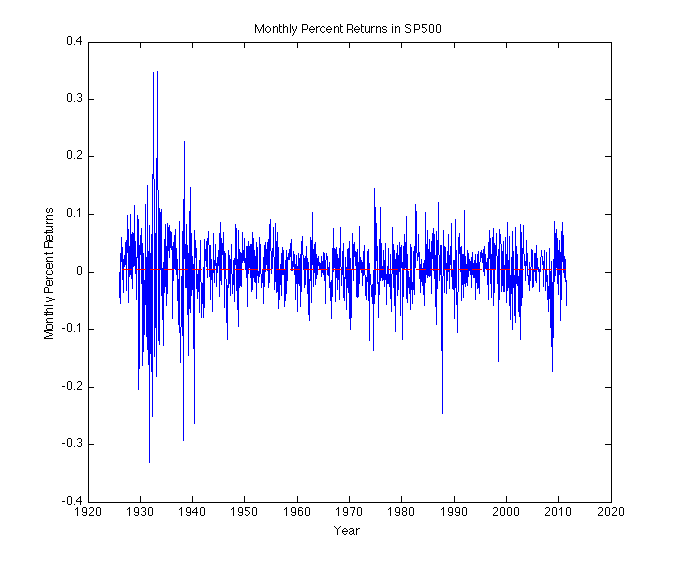
\includegraphics[scale=0.4]{Figures/Sp500MonthlyReturns}
\end{figure}
\end{frame}

\begin{frame}
\frametitle[alignment=center]{Motivating functional form-III}
\begin{figure}
\centering
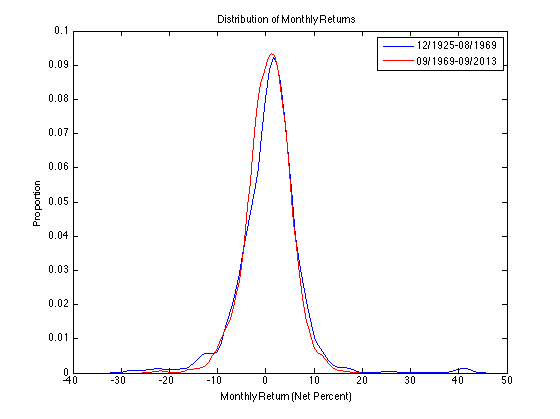
\includegraphics[scale=0.5]{Figures/DistributionofReturns}
\end{figure}
\end{frame}

\begin{frame}
\frametitle[alignment=center]{Motivating functional form-IV}
\begin{figure}
\centering
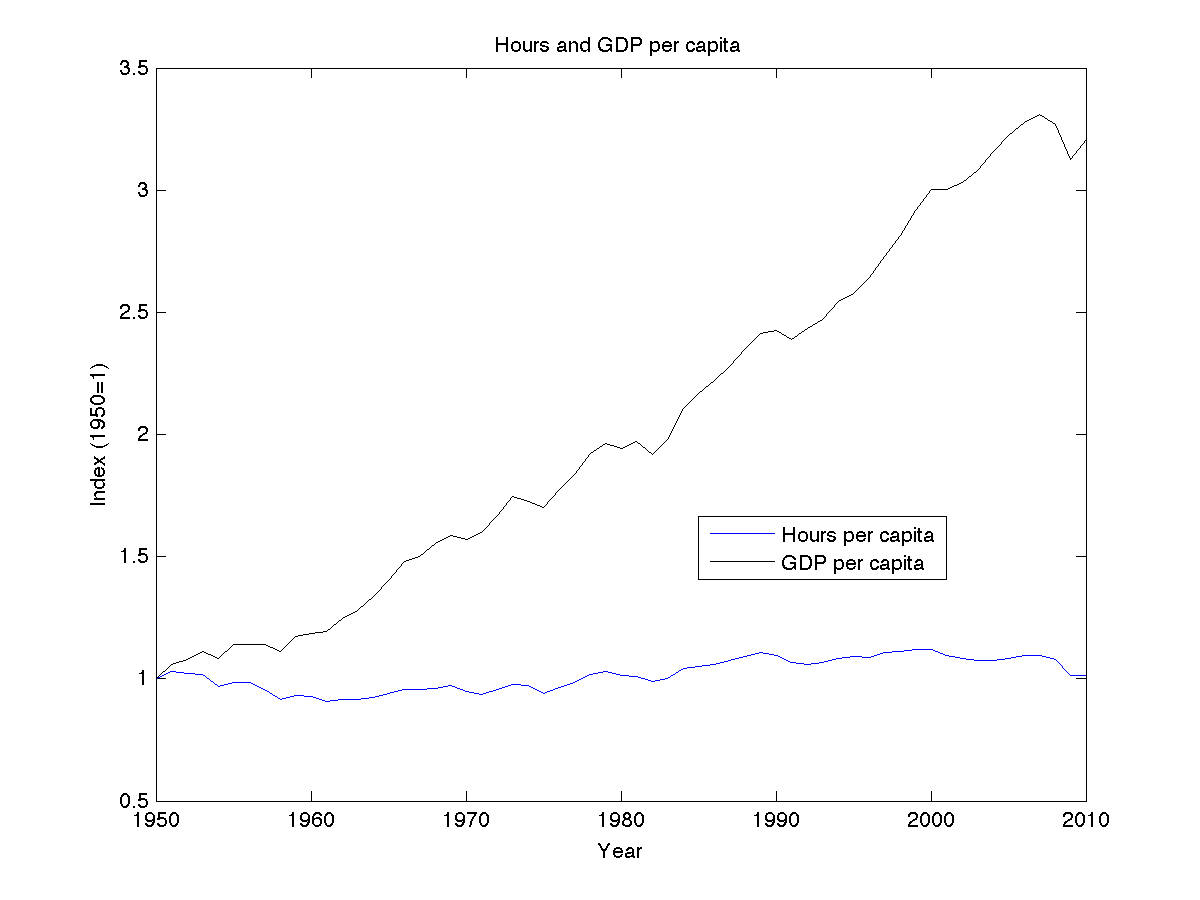
\includegraphics[scale=0.25]{Figures/HoursandGDP}
\end{figure}
\end{frame}

\begin{frame}
\frametitle[alignment=center]{Motivating functional form-V}
\begin{figure}
\centering
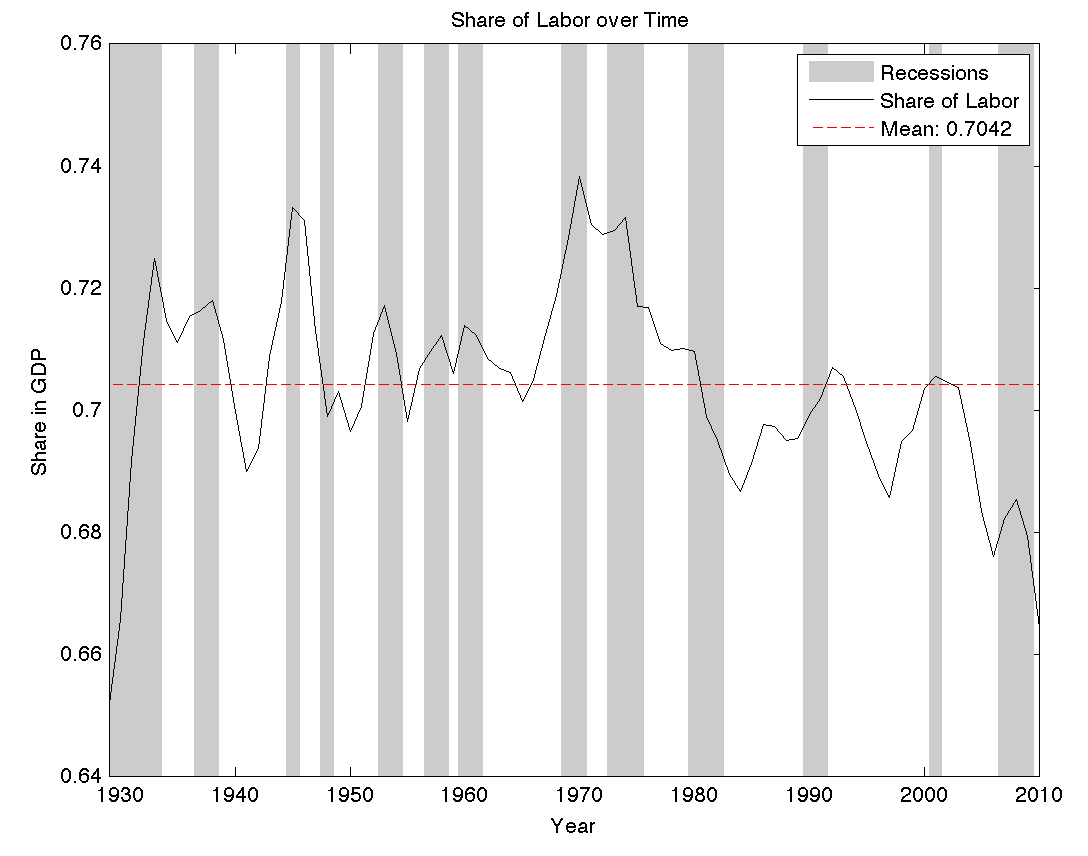
\includegraphics[scale=0.25]{Figures/LaborShare}
\end{figure}
\end{frame}

\begin{frame}
\frametitle[alignment=center]{Motivating functional form-VI}
\begin{figure}
\centering
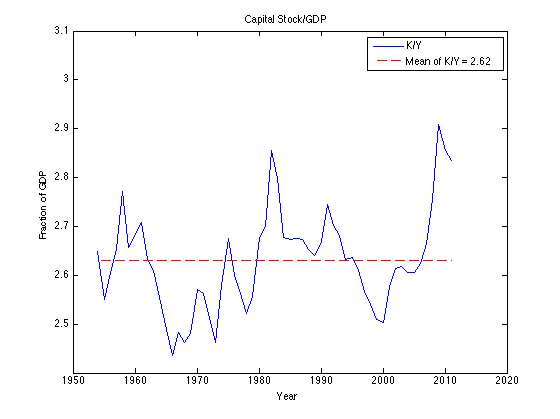
\includegraphics[scale=0.5]{Figures/KoverY}
\end{figure}
\end{frame}

\begin{frame}
\frametitle[alignment=center]{Discipline Functional Form}
\begin{itemize}
\item Stylized/Kaldor's facts (per capita!):
\begin{itemize}
\item $Y_t,C_t,K_t,w_t$ have grown at a constant rate
\item $r_t,L_t$ have not.
\item $(r_t-\delta)K_t/Y_t$, $w_tL_t/Y_t$ have been constant.
\end{itemize}
\item This gives utility you normally see:
$$u(C_t,1-L_t)=\frac{(C_t\cdot g(1-L_t))^{1-\sigma}-1}{1-\sigma}$$
or
$$u(C_t,1-L_t) = \log(C_t)+\psi \log(1-L_t)$$
or:
$$u(C_t,1-L_t) = \log(C_t)-\psi \frac{\epsilon}{1+\epsilon}L_t^{\frac{1+\epsilon}{\epsilon}}$$
\item And production:
$$Y_t=A_t\left(\xi K_t^\frac{\sigma-1}{\sigma}+(1-\xi) L_t^\frac{\sigma-1}{\sigma}\right)^\frac{\sigma}{\sigma-1}$$
or:
$$Y_t=A_tL_t^\alpha K_t^{1-\alpha}$$
\end{itemize}
\end{frame}

\begin{frame}
\frametitle[alignment=center]{Simple NCG}
$$\max\sum_{t=0}^\infty \beta^t\left[\log(c_t)+\psi\left(1-L_t\right)\right]$$
\bigskip
$$C_t+I_t=A_tK_t^\alpha L_t^{1-\alpha}$$
\bigskip
$$K_{t+1}=(1-\delta)K_t+I_t$$
\end{frame}

\begin{frame}
\frametitle[alignment=center]{Simple NCG: FOC's}
Given $K_0$, each period has 6 equations and 6 unknowns ($C_{t},K_{t+1},L_t,Y_t,w_t,r_t$)
$$\begin{array}{rclcl}
\frac{C_{t+1}}{C_t} & = & \beta(1-\delta+r_{t+1}) & \ \ \  & \text{Euler/intertemporal/$K^S$} \\
\frac{\psi}{1-L_t} & = & \frac{w_t}{C_t} &  \ \ \  & \text{Intratemporal/$L^S$}\\
w_t & = & (1-\alpha)\frac{Y_t}{L_t} &  \ \ \ & \text{$L^D$}\\
r_t & = & \alpha\frac{Y_t}{K_t} &  \ \ \ & \text{$K^D$}\\
K_{t+1} & = & (1-\delta)K_t+I_t &  \ \ \ &  \text{Law of motion of capital}\\
I_t+C_t & = & Y_t &  \ \ \ & \text{Feasibility} \\
\uncover<2->{w_tL_t+r_tK_t & = & C_t+I_t & & \text{Budget constraint} \\}
\end{array}$$
\uncover<2->{Extra equation?}\\
\ \\
\uncover<3->{Can reduce to two series.}
\end{frame}

\begin{frame}
\frametitle[alignment=center]{Bring the model to data: issues?}
\begin{itemize}
\item $Y_t\neq I_t+C_t$!
\bigskip
\begin{itemize}
\item $Y_t\neq I_t+C_t+G_t+(I_t-X_t)$!  
\bigskip
\item Could try to divvy up $G$ and $NX$
\bigskip
\item Could attribute all to $C$
\bigskip
\item Does it matter?  
\end{itemize}
\bigskip
\item One type of capital
\bigskip
\item One price for everything (constant relative price of capital and consumption)
\bigskip
\item No terms of trade
\bigskip
\item Need to calibrate parameters: $\beta$, $\delta$, $K_0$, $\psi$, $\alpha$, and $A_t$'s
\end{itemize}
\end{frame}

\begin{frame}
\frametitle[alignment=center]{Bring the model to data: Step 1}
\begin{itemize}
\item Calibrate: $\beta$, $\delta$, $K_0$, $\psi$, $\alpha$, and $A_t$'s
\item Given $I_t$ data and $\delta K_t$ data, choose $\delta$ and $K_0$ to target:
$$\underbrace{\overline{\frac{\delta K_t}{Y_t}}}_{Data}=\underbrace{\overline{\frac{\delta K_t}{Y_t}}}_{Model}$$
And:
$$\frac{ K_1}{Y_1}=\frac{1}{10}\sum_{t=1}^{10}\frac{K_t}{Y_t}$$
That is, average depreciation in the model is the same as average depreciation in the data, and the starting capital/output ratio is comparable to the capital/output ratio over the next 10 periods.
\item Calibrate: $\beta$, $\cancel{\delta}$, $\cancel{K_0}$, $\psi$, $\alpha$, and $A_t$'s
\end{itemize}
\end{frame}

\begin{frame}
\frametitle[alignment=center]{Bring the model to data: Step 2}
\begin{itemize}
\item Given $K_0$ and $\delta$, along with $I_t$, can construct $K_t$'s in data
\item Given constructed $K_t$, $L_t$ and $Y_t$ in data, can calculate TFP:
$$A_t=\frac{Y_t}{L_t^\alpha K_t^{1-\alpha}}$$ 
\item Can calibrate $\alpha$ as the average wage share:
$$\alpha = \frac{1}{N}\sum_{t=1}^N\frac{w_tL_t}{Y_t}$$
\item Calibrate: $\beta$, $\cancel{\delta}$, $\cancel{K_0}$, $\psi$, $\cancel{\alpha}$, and $\cancel{A_t}$'s
\end{itemize}
\end{frame}

\begin{frame}
\frametitle[alignment=center]{Bring the model to data: Step 3}
\begin{itemize}
\item Set $\beta$ so that the \emph{expectation} of the intertemporal FOC in the data is true.
$$\beta=\frac{1}{N}\sum_{t=1}^N\frac{1}{(1-\delta+r_{t+1})}\frac{C_{t+1}}{C_t}$$
\item Set $\psi$ so that the \emph{expectation} of the intratemporal FOC in the data is true.
$$\psi = \frac{1}{N}\sum_{t=1}^N\frac{w_t(1-L_t)}{C_t} $$
\item Calibrate: $\cancel{\beta}$, $\cancel{\delta}$, $\cancel{K_0}$, $\cancel{\psi}$, $\cancel{\alpha}$, and $\cancel{A_t}$'s
\end{itemize}
\end{frame}

\begin{frame}
\frametitle[alignment=center]{So actually take it to data}
\begin{itemize}
\item I'm just going to use BEA data
\bigskip
\item Download GDP $(Y_t)$, Personal Consumption $(C_t)$ from Table 1.1.6
\bigskip
\item Download Gross Domestic Investment $I_t$ and consumption of fixed capital $\delta K_t$ from Table 5.2.6.
\bigskip
\item Download Population from Table 7.1
\bigskip
\item Download Hours and Employment from OECD
\bigskip
\item Let's look at the series
\end{itemize}
\end{frame}

\begin{frame}
\frametitle[alignment=center]{GDP, Investment, Consumption, Labor hours}
\begin{figure}
\centering
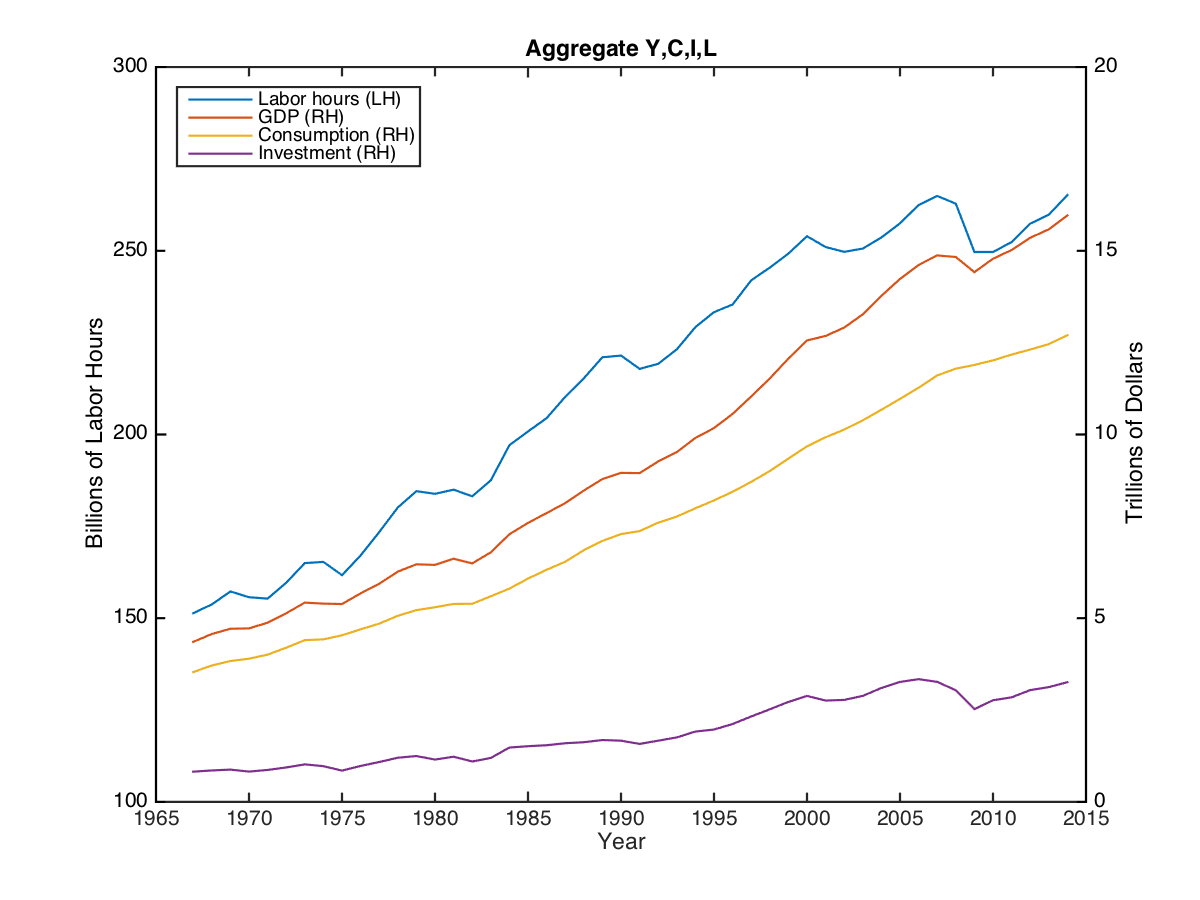
\includegraphics[scale=0.5]{Figures/Figure_1.png}
\end{figure}
\end{frame}

\begin{frame}
\frametitle[alignment=center]{Per Capita}
\begin{figure}
\centering
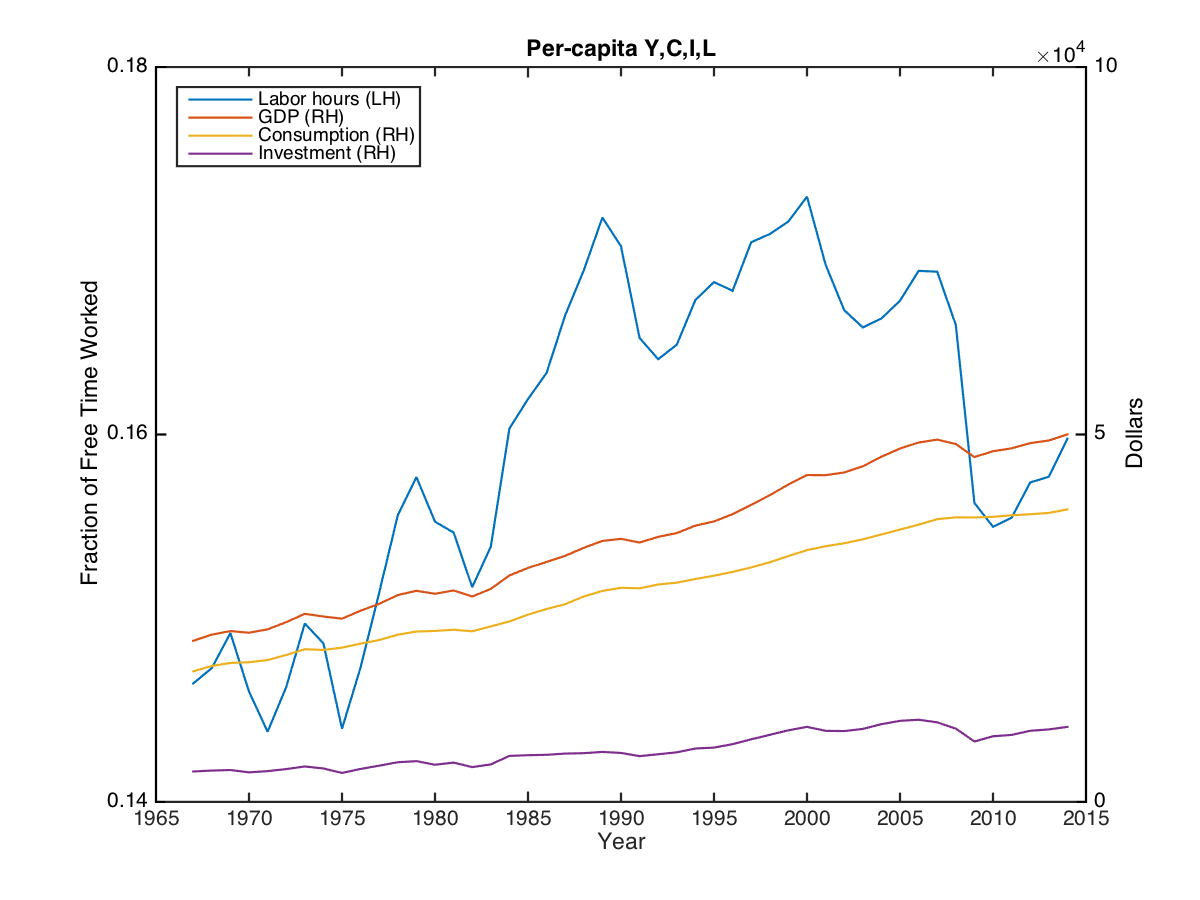
\includegraphics[scale=0.5]{Figures/Figure_2.png}
\end{figure}
\end{frame}

\begin{frame}
\frametitle[alignment=center]{Create Capital Stock}
\begin{figure}
\centering
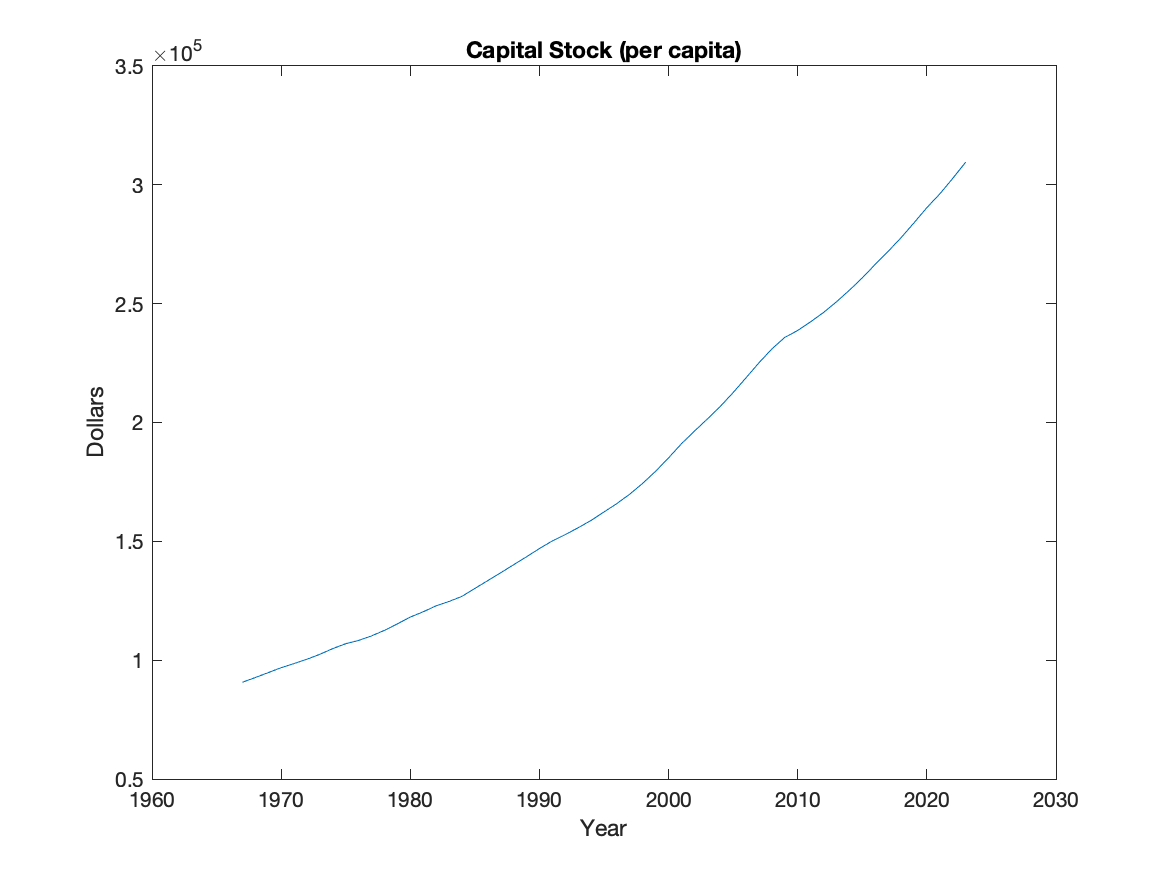
\includegraphics[scale=0.5]{Figures/Figure_3.png}
\end{figure}
\end{frame}

\begin{frame}
\frametitle[alignment=center]{Create Capital Stock: $K_{t+1}=(1-\delta)K_t+I_t$}
\begin{figure}
\centering
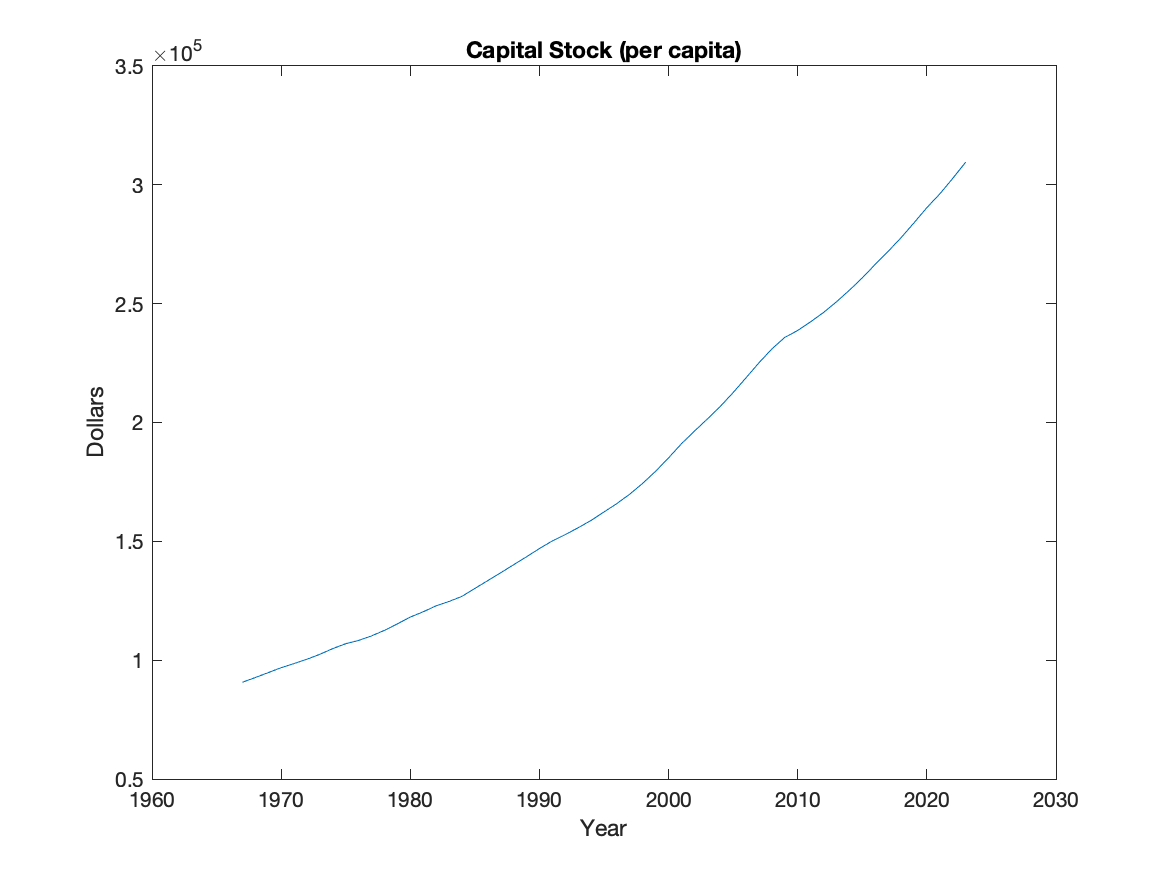
\includegraphics[scale=0.5]{Figures/Figure_3.png}
\end{figure}
\end{frame}

\begin{frame}
\frametitle[alignment=center]{Find TFP: $A_t=\frac{Y_t}{L_t^\alpha K_t^{1-\alpha}}$}
\begin{figure}
\centering
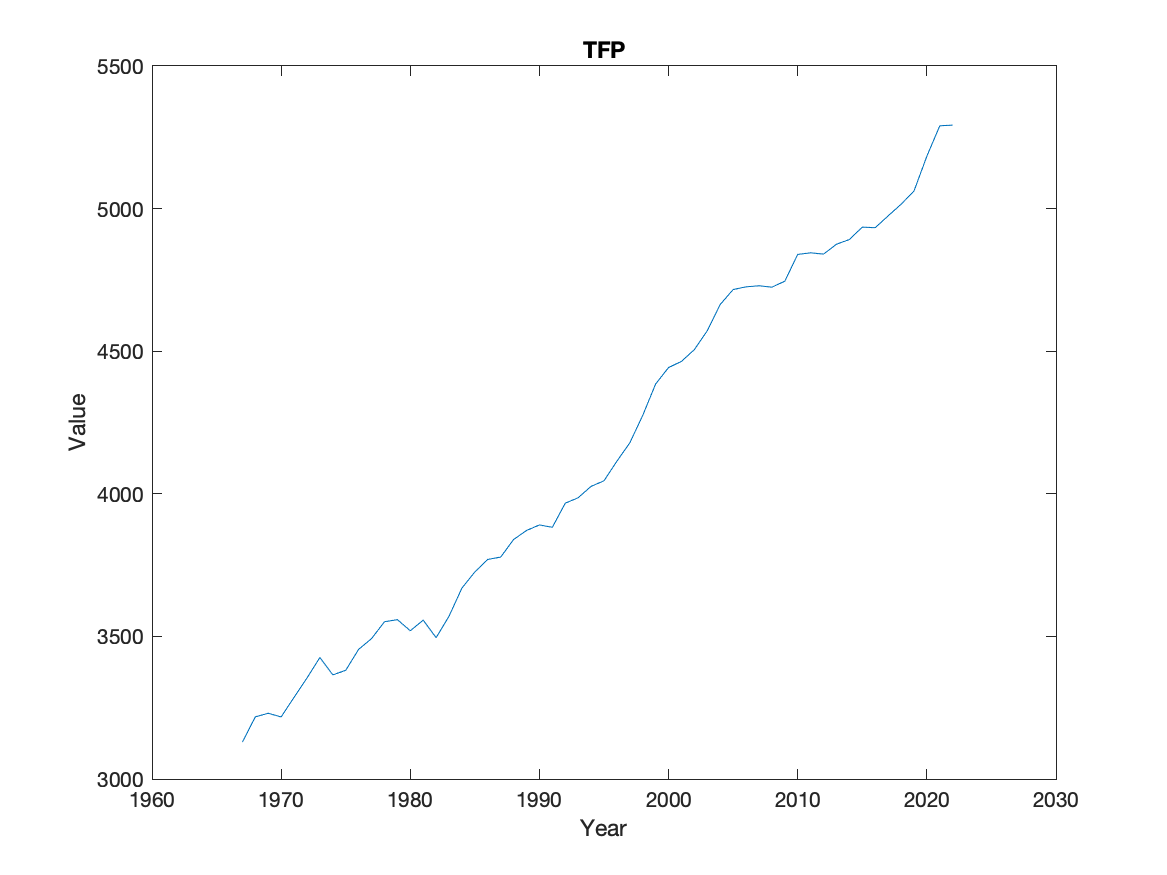
\includegraphics[scale=0.5]{Figures/Figure_4.png}
\end{figure}
\end{frame}

\begin{frame}
\frametitle[alignment=center]{Find $\beta=\frac{1}{1-\delta+r_{t+1}}\frac{c_{t+1}}{c_t}$}
\begin{figure}
\centering
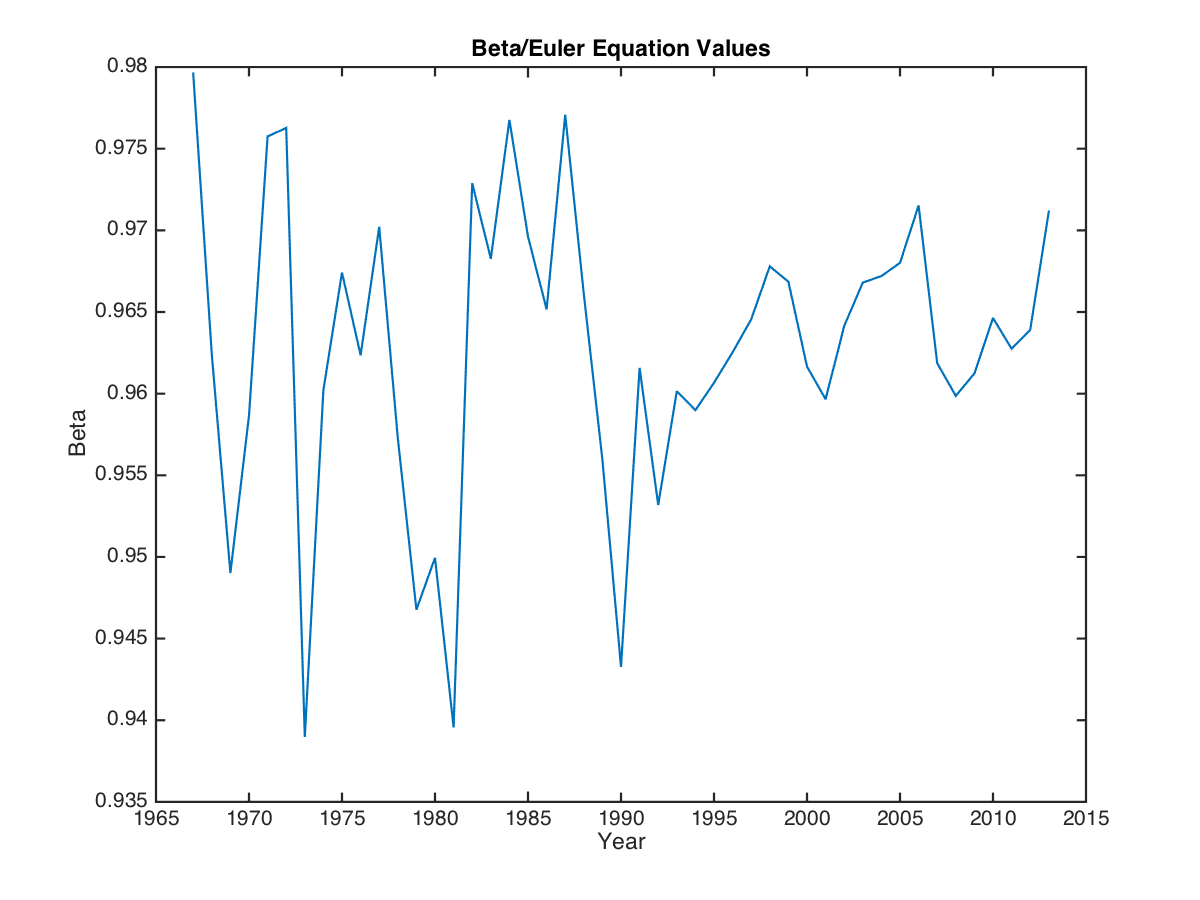
\includegraphics[scale=0.5]{Figures/Figure_5.png}
\end{figure}
\end{frame}

\begin{frame}
\frametitle[alignment=center]{Find $\psi=\frac{w_t(1-L_t)}{c_t}$}
\begin{figure}
\centering
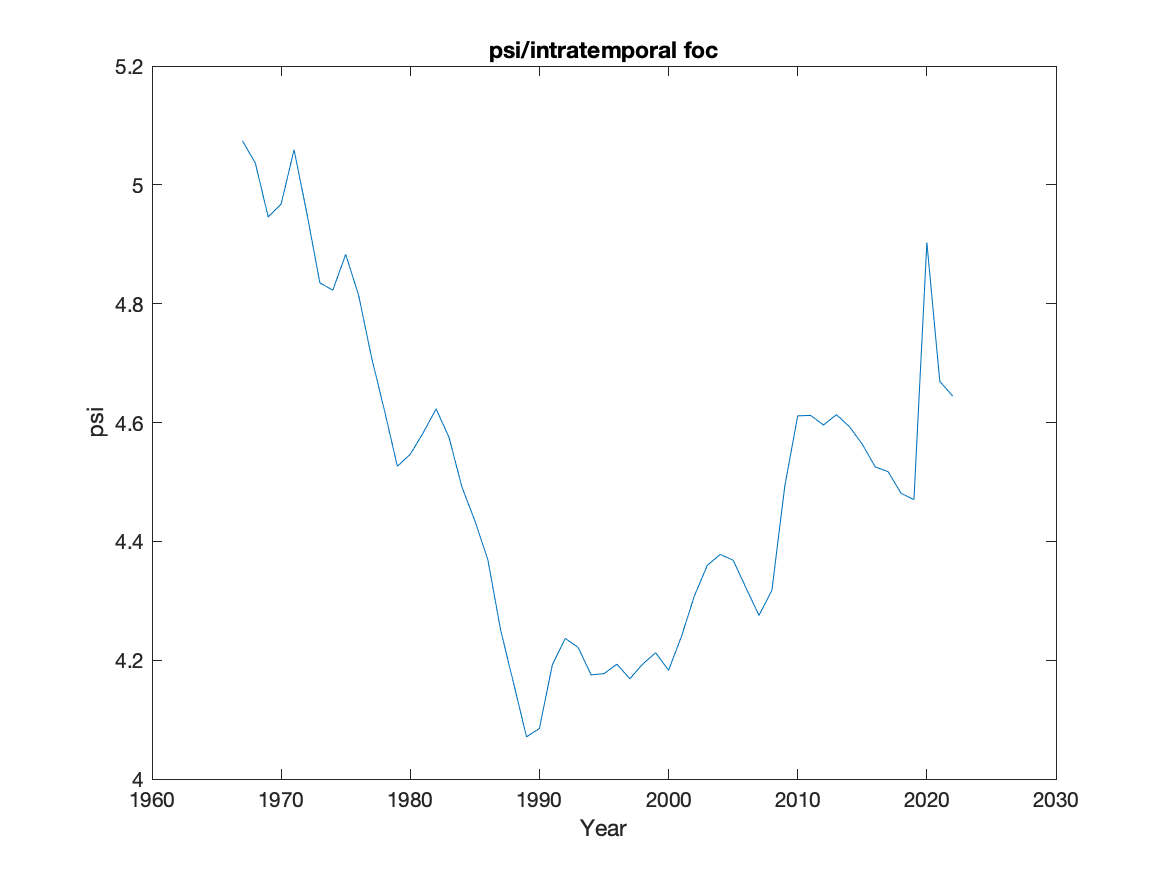
\includegraphics[scale=0.5]{Figures/Figure_6.png}
\end{figure}
\end{frame}

\begin{frame}
\frametitle[alignment=center]{Calibration}
\begin{itemize}
\item $k_0=63396$
\bigskip
\item $\delta=0.043$
\bigskip
\item $\beta=0.963$
\bigskip
\item $\psi=4.58$
\bigskip
\item $\alpha=0.7$
\end{itemize}
\end{frame}

\begin{frame}
\frametitle[alignment=center]{Solution and Assumptions}
\begin{itemize}
\item There are many possible assumptions with respect to $A_t$
\bigskip
\item A first step is complete knowledge of $A_t$
\bigskip
\item Assume no labor, consumption, or capital taxes
\bigskip
\item What about future $A_t$?
\bigskip
\item Continue $A_t$ growth constantly into the future
\bigskip
\item Force to reach steady state growth path 20 years into constant future
\end{itemize}
\end{frame}

\begin{frame}
\frametitle[alignment=center]{Solution Method}
\begin{itemize}
\item Given parameters, a path of $A_t$, and a $k_0$, I have two decisions to make:
\bigskip
\begin{itemize}
\item $L_t\times T$ labor decisions from intratemporal FOC
\bigskip
\item $K_{t+1}\times T$ capital decisions from intertemporal FOC
\bigskip
\end{itemize} 
\item Solve for 40 existing years, then give 30 years to reach SS growth path
\bigskip
\item Then, for 30 more periods, assume they're on autopilot
\bigskip
\item They only get to choose $70\times 2$ choices to solve $70\times2+30\times2$ FOC's!
\bigskip
\item Make sure all FOC's are zero
\end{itemize}
\end{frame}


\begin{frame}
\frametitle[alignment=center]{Theory and Data}
\begin{figure}
\centering
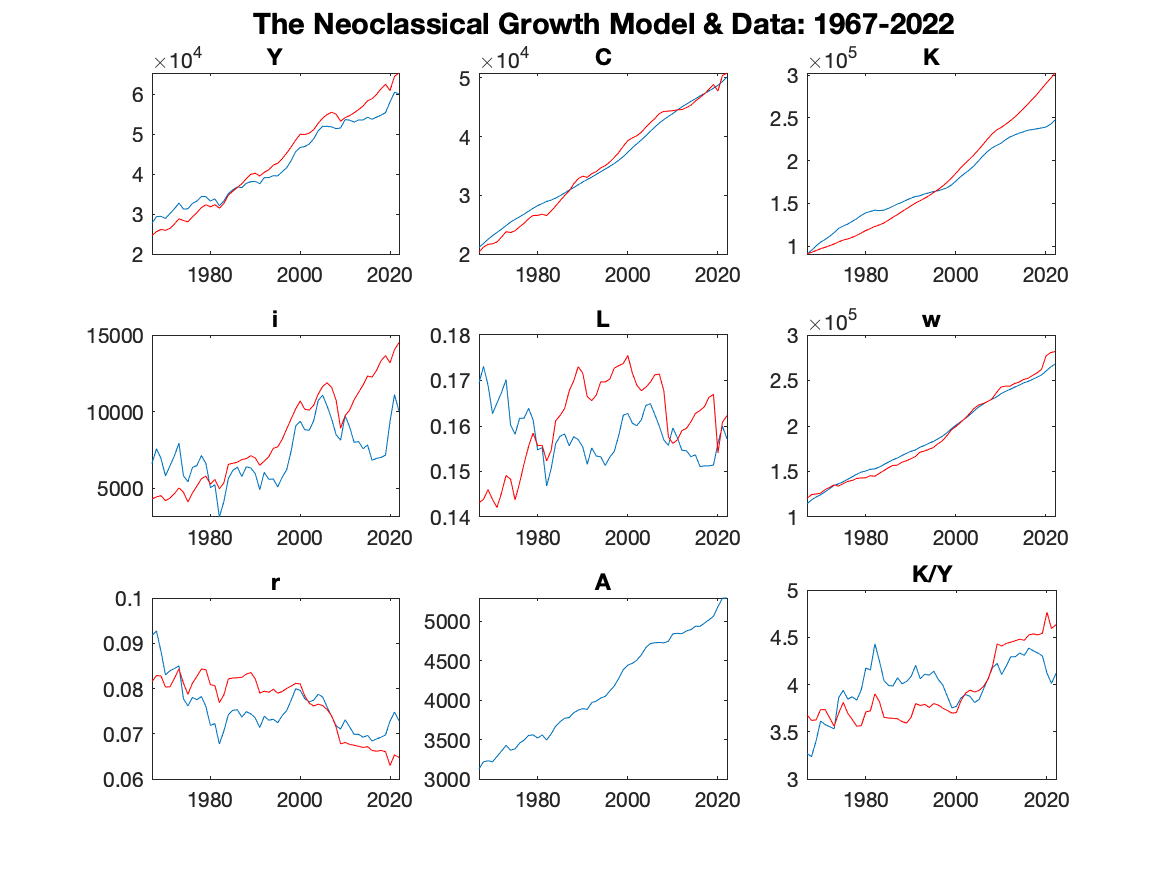
\includegraphics[scale=0.5]{Figures/Figure_7.png}
\end{figure}
\uncover<2->{Which is theory, which is data?}
\end{frame}

\begin{frame}
\frametitle[alignment=center]{Explaining the early 1980's}
\begin{figure}
\centering
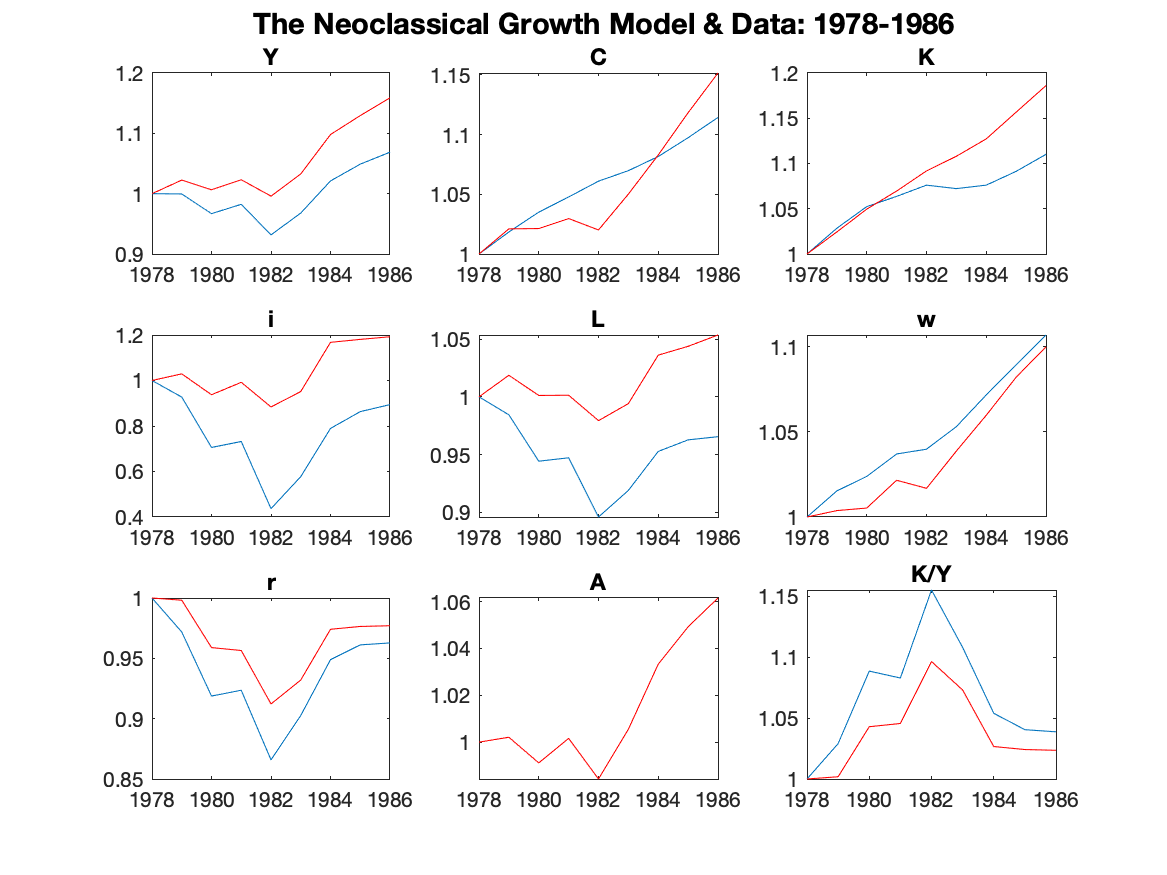
\includegraphics[scale=0.5]{Figures/Figure_8.png}
\end{figure}
\end{frame}


\begin{frame}
\frametitle[alignment=center]{Explaining the late 2000's}
\begin{figure}
\centering
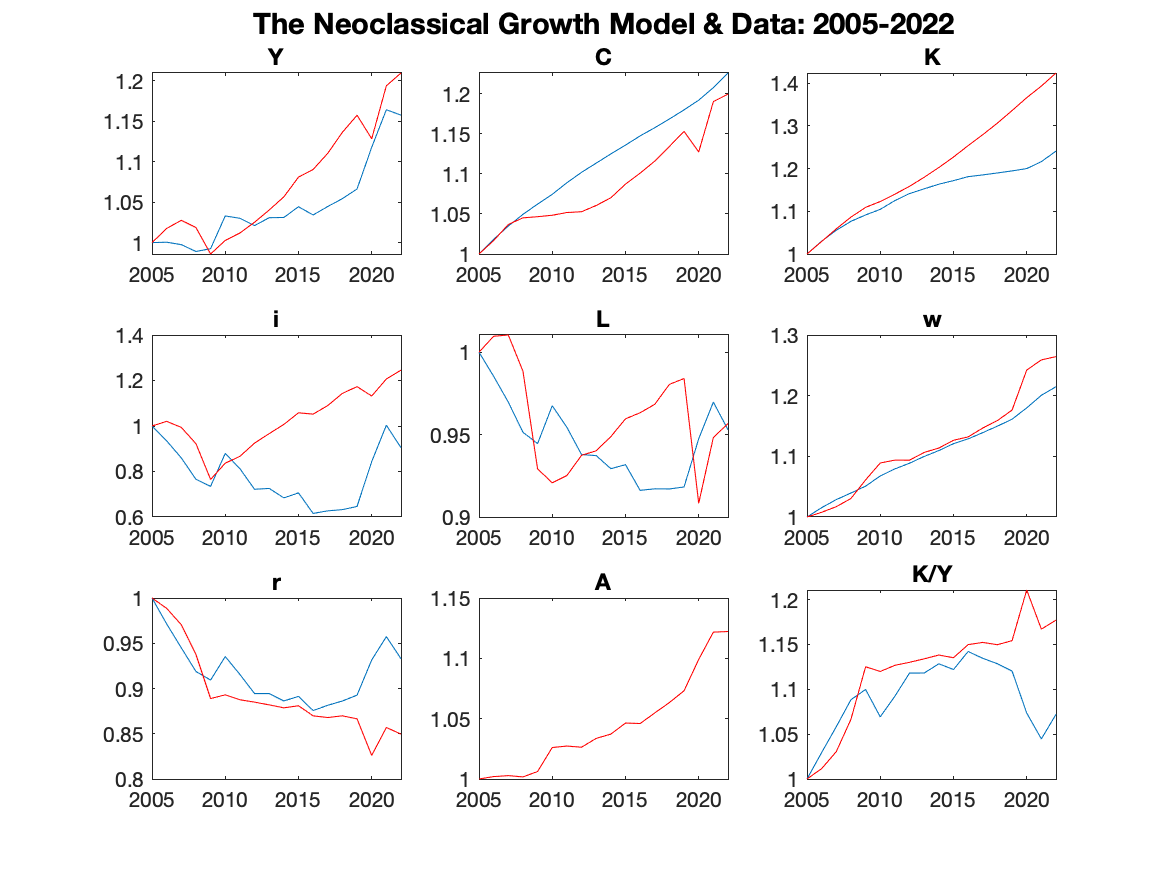
\includegraphics[scale=0.5]{Figures/Figure_9.png}
\end{figure}
\end{frame}


\begin{frame}
\frametitle[alignment=center]{(Macro)Economics as a science}
\begin{itemize}
\item In similar position to meteorology, astronomy, geology
\bigskip
\item No randomized experiments
\bigskip
\item Data is too short for nonparametric analysis
\bigskip
\item Ideal (and solution) a unified theory: explain all frequencies
\bigskip
\item Parsimony keeps us honest
\bigskip
\item Explaining multiple stochastic processes jointly keeps us honest
\bigskip
\item Explaining dynamics gives more role for testable hypotheses
\end{itemize}
\end{frame}


\end{document}